\documentclass{article}
\usepackage[utf8]{inputenc}
\usepackage{a4wide}
\usepackage{dsfont}
\usepackage{upgreek}
\usepackage{setspace} \doublespacing
\usepackage{mathtools}
\usepackage{titlesec}
\usepackage[]{biblatex}
\usepackage{xcolor}
\usepackage{graphicx}
\usepackage[]{amsmath,amssymb,amsfonts, amsthm}
\usepackage{geometry}
\usepackage{breqn}
\usepackage{multicol}
\usepackage{tikz}
\usepackage{mathdots}
\usepackage{color}
\usetikzlibrary{fadings}
\usetikzlibrary{patterns}
\usetikzlibrary{shadows.blur}
\usetikzlibrary{shapes}
\usetikzlibrary{automata, arrows.meta, positioning}
\title{\textbf{Tutorial solutions (Part-II)}}
\author{Om Swostik Mishra, Anish Kulkarni}
\date{}
\begin{document}
\maketitle
\tableofcontents
\clearpage
\begin{flushleft}
\section{Tutorial-1}
\textbf{1}:\\
Given $\phi= \forall x\exists y \:R(x,y)\: \wedge\: \exists y \forall x\:\neg R(x,y)$.\\
Take the model to be the set of naturals $\mathbb{N}$ with $<$ relation.\\
Then, $m\models \phi$ (Why?)\\
(\textbf{Hint}: $\mathbb{N}$ is an well-ordered set (i.e has a minimum) and isn't bounded above)\\
\textbf{2}:\\
$\varphi_B(x,y)=\exists z(P(z,x)\wedge P(z,y))\wedge \neg F(x)$\\
$\varphi_A(x,y)=\exists z(P(z,y)\wedge \varphi_S(x,z))$   \hspace{4.5mm} ($\varphi_S(x,y)=\exists z(P(z,x)\wedge P(z,y))\wedge F(x)$, $x$ is sister of $y$)\\
$\varphi_C(x,y)=\exists z(\varphi_A(z,x)\wedge P(z,y))$\\
$\varphi_O(x)=\forall z,y (P(z,y)\wedge P(z,x)\Rightarrow (x=y))$\\
The spousal relationship cannot be defined (Why?)\\
\textbf{3}:\\
$Zero(x)=\:+(x,x)=x$\\
$One(x)= \forall y(\times(x,y)=y)$\\
$Two(x)= \exists z((+(z,z)=x)\wedge One(z))$\\
$Even(x)= \exists z,y((\times(z,y)=x)\wedge Two(y))$ \\
$Odd(x)=\neg Even(x)$\\
$Prime(x)= \neg One(x)\wedge (\neg \exists w,y((\times(w,y)=x)\wedge(\neg One(w)\wedge \neg One(y))))$\\
Goldbach conjecture in FO: $\forall x(\neg One(x)\wedge \neg Two(x)\wedge Even(x)\Rightarrow \exists z,w(Prime(z)\wedge Prime(w)\wedge +(z,w)=x))$\\
\textbf{4}:\\
Encoding associativity of $+$:  $\forall x,y,z(+(x,+(y,z))=+(+(x,y),z))$\\
Encoding the right identity as $0$:  $\forall x(+(x,0)=x)$\\
Encoding right inverse: $\forall x\exists y(+(x,y)=0)$\\
Encoding A(4): $\forall x,y,z(+(x,z)=+(y,z)\Rightarrow x=y)$\\
Here we have used the signature $\tau=(0,+)$.\\
\textbf{5}:\\
\textbf{(i)} Consider the set of integers $\mathbb{Z}$ with the induced relation $+_Z$ referring to the usual addition in $\mathbb{Z}$. The constant $0_Z$ refers to $0$ in $\mathbb{Z}$. Observe that addition is associative and admits both left and right inverses. Also $0$ is a identity for addition.
We can conclude the $\tau$-structure $\mathbb{Z}$ satisfies $\psi$.\\
\textbf{(ii)} Consider the set $\mathbb{N}_0$ of whole numbers and the corresponding induced relation being addition and the constant being $0$ (in $\mathbb{N}_0$). This $\tau$-structure doesn't satisfy $\psi$ as $\varphi_3$ fails to be true (non-zero elements in $\mathbb{N}_0$ don't have inverses).\\
\textbf{(iii)} Consider the set of all $n\times n$ invertible matrices with complex values, $GL_n(\mathbb{C})$. Let the induced binary operation be matrix multiplication and let the constant $0$ map to the identity $n\times n$ matrix.\\
It's clear that the $\tau$-structure $GL_n(\mathbb{C})$ satisfies $\psi$, however, it doesn't satisfy $\forall x,y(+(x,y)=+(y,x))$ (Why?).\\
\textbf{(iv)} As before, consider the set $\mathbb{N}_0$ of whole numbers with the usual addition. This satisfies $\varphi_1\wedge\varphi_2$ but doesn't satisfy $\varphi_3$.\\
Consider the set of non-negative reals $\mathbb{R}_{\geq0}$, with the binary operation defined as $+(a,b)=|a-b|$ and the constant mapping to $0$. Show that this structure satisfies $\varphi_2\wedge \varphi_3$ but fails to satisfy $\varphi_1$.\\
Consider $\mathbb{Z}$ with the usual addition and the constant $0$ mapping to $1$ (in $\mathbb{Z}$). This satisfies $\varphi_1\wedge\varphi_3$ but fails to satisfy $\varphi_2$.\\
We can conclude that $\psi$ isn't equivalent to any of $\varphi_1\wedge\varphi_2$, $\varphi_2\wedge\varphi_3$ or $\varphi_1\wedge\varphi_3$.
\clearpage
\textbf{7}:

\tikzset{every picture/.style={line width=0.75pt}} %set default line width to 0.75pt        

\begin{tikzpicture}[x=0.75pt,y=0.75pt,yscale=-1,xscale=1]
%uncomment if require: \path (0,300); %set diagram left start at 0, and has height of 300

%Shape: Circle [id:dp8408479190255029] 
\draw   (100,138) .. controls (100,124.19) and (111.19,113) .. (125,113) .. controls (138.81,113) and (150,124.19) .. (150,138) .. controls (150,151.81) and (138.81,163) .. (125,163) .. controls (111.19,163) and (100,151.81) .. (100,138) -- cycle ;
%Shape: Circle [id:dp750067727127359] 
\draw   (290,59) .. controls (290,45.19) and (301.19,34) .. (315,34) .. controls (328.81,34) and (340,45.19) .. (340,59) .. controls (340,72.81) and (328.81,84) .. (315,84) .. controls (301.19,84) and (290,72.81) .. (290,59) -- cycle ;
%Shape: Circle [id:dp24092758810894677] 
\draw   (292.33,227.17) .. controls (292.33,213.45) and (303.45,202.33) .. (317.17,202.33) .. controls (330.88,202.33) and (342,213.45) .. (342,227.17) .. controls (342,240.88) and (330.88,252) .. (317.17,252) .. controls (303.45,252) and (292.33,240.88) .. (292.33,227.17) -- cycle ;
%Straight Lines [id:da33436515075759754] 
\draw    (148.33,147) -- (294.33,217) ;
%Straight Lines [id:da7853123539498421] 
\draw    (149.33,129) -- (290,59) ;
%Curve Lines [id:da8590354572311187] 
\draw    (102.33,127) .. controls (43.33,100) and (41.33,176) .. (103.33,153) ;
%Curve Lines [id:da3623243093402584] 
\draw    (338.33,47) .. controls (390.33,30) and (410.33,89) .. (336.33,72) ;
%Curve Lines [id:da6684122826682815] 
\draw    (338.33,215) .. controls (378.33,185) and (420.33,248) .. (340.33,241) ;

% Text Node
\draw (120,132) node [anchor=north west][inner sep=0.75pt]   [align=left] {A};
% Text Node
\draw (311,52) node [anchor=north west][inner sep=0.75pt]   [align=left] {B};
% Text Node
\draw (311,220) node [anchor=north west][inner sep=0.75pt]   [align=left] {C};


\end{tikzpicture}\\
\vspace{2mm}
Consider the undirected graph $\mathcal{G}$ above (with loops). This (with its natural edge relation) satisfies the second formula but not the first.\\
\textbf{8}: \\$\exists^{\geq n}x(x=x)\:\wedge\:\neg\exists ^{\geq n+1}x(x=x)$ is true for all models whose universe has exactly $n$ elements.\\
Let $\varphi= \exists x_1, x_2\dots x_n(\wedge^{}_{i\neq j}(x_i\neq x_j))$.\\
$\varphi \equiv \exists^{\geq n}x(x=x)$ (Why?)\\
\textbf{9}:\\
Using counting quantifiers, we can write,\\
$\varphi= \exists^{\geq n}x(x=x)\:\wedge\:\neg\exists ^{\geq m+1}x(x=x)$\\
$\varphi$ evaluates to true only over models with atleast $n$ and atmost $m$ elements.
\section{Tutorial-2}
\textbf{1:}\\
\textbf{(a)} Observe that this is the same as the set of the words that start and end in the same letter! (Try and see how. A hint: An ``\textit{ab}" occurrence can be seen as ``switching" from \textit{a} to \textit{b} while parsing the word from left to right. Similar for ``\textit{ba}".)
We'll define the following functions w.r.t the word signature - they'll help us out throughout the tutorial:\newline
$\hspace{1cm} first(x) = \forall y.(x < y \lor x = y) \hspace{4cm}
last(x) = \forall y.(x > y \lor x = y)$ \\
So, $\varphi_1 = \exists x.(\;\exists y.(\;first(x) \land last(y) \land \neg(Q_a(x) \land Q_b(y)) \land \neg(Q_b(x) \land Q_a(y))\;)\;)$ is s.t. $L(\varphi_1) = L$.

\textbf{(b)} $\varphi_2 = \exists x.(\;Q_\#(x) \land \forall y.(\;(x < y \Rightarrow Q_b(y)) \land (y < x \Rightarrow Q_a(y))\;)\;)$ is such that $L(\varphi_2) = L$.\\
Note - for any letter in our alphabet we have its corresponding $Q$-function - hence, $Q_\#$ in our $\varphi_2$.

\textbf{(c)} Either there is no $b$ or the only $b$'s in the word come at the end.\\
Hence, $\varphi_3 = \forall x \forall y.(\; (S(x,\, y) \land Q_b(x)) \Rightarrow Q_b(y)\;)$ is such that $L(\varphi_3) = L$.

\textbf{(d)} $\varphi_4 = \exists x \exists y.(\; first(x) \land last(y) \land \forall z.(\; (S(x, z) \lor S(z, y)) \Rightarrow Q_0(z)\;)\;)$ is s.t. $L(\varphi_4) = L$.

\textbf{(e)} Say we parse the word letters from left to right. In the beginning, the top and bottom entries of each letter may or may not be the same. However, if we want the top row to be larger than the bottom row, then the moment where the entries first differ will be $1 \choose 0$.\\ 
Hence, $\varphi_5 = \exists x.(\;Q_{1 \choose 0}(x) \land \forall y.(\; y < x \Rightarrow (Q_{0 \choose 0}(y) \lor Q_{1 \choose 1}(y))\;)\;)$ is s.t. $L(\varphi_5) = L$.

\textbf{2:}\\

Note that for all $\varphi$, $L(\varphi)$ is by definition FO-definable, and hence regular. This is as \textit{FO-definable languages $\subseteq$ regular languages}. (How? Given an FO formula, can we find an algorithm to construct a DFA for its language?). Also, as regular languages are closed under complementation, $\overline{L(\varphi)}$ will also be regular. 

\textbf{(1)} $L(\varphi) = {\epsilon}.$ The DFA is given by:\vspace{3mm}

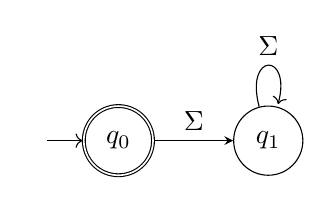
\begin{tikzpicture}
    \node (q0) [state, initial, accepting, initial text = {}] {$q_0$};
    \node (q1) [state, right = of q0] {$q_1$};
    \path [-stealth]
        (q0) edge node[above] {$\Sigma$} (q1)
        (q1) edge[loop above] node[above] {$\Sigma$} (); 
\end{tikzpicture} \\
Naturally, only a structure (model) with an empty universe (domain) can satisfy $\varphi$ here.

\textbf{(2)} $L(\varphi) = \Sigma^* b a^* a \Sigma^*$. The DFA is given by:\vspace{3mm}

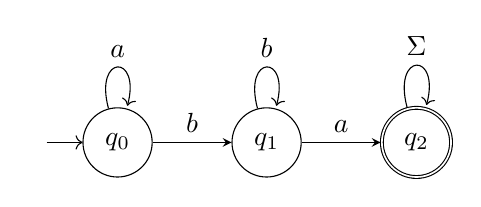
\begin{tikzpicture}
    \node (q0) [state, initial, initial text = {}] {$q_0$};
    \node (q1) [state, right = of q0] {$q_1$};
    \node (q2) [state, accepting, right = of q1] {$q_2$};
    \path [-stealth]
        (q0) edge [loop above] node {$a$}()
        (q0) edge node[above] {$b$} (q1)
        (q1) edge [loop above] node {$b$}()
        (q1) edge node[above] {$a$} (q2)
        (q2) edge [loop above] node {$\Sigma$}();
\end{tikzpicture}\\
Observe that we need to encode $an$ occurrence of $b a^* a$. With the first 2 states, we are basically encoding the $first$ such occurrence.

\textbf{(3)} $L(\varphi) = \Sigma^* a \Sigma$. The DFA is given by:\vspace{3mm}

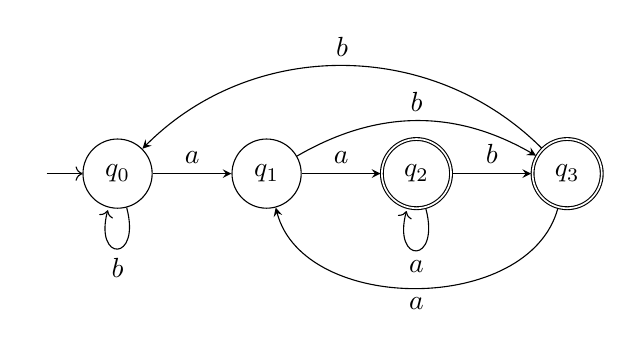
\begin{tikzpicture}
    \node (q0) [state, initial, initial text = {}] {$q_0$};
    \node (q1) [state, right = of q0] {$q_1$};
    \node (q2) [state, accepting, right = of q1] {$q_2$};
    \node (q3) [state, accepting, right = of q2] {$q_3$};
    \path [-stealth]
        (q0) edge [loop below] node {$b$}()
        (q0) edge node[above] {$a$} (q1)
        (q1) edge node[above] {$a$} (q2)
        (q1) edge[bend left] node[above] {$b$} (q3)
        (q2) edge [loop below] node {$a$}()
        (q2) edge node[above] {$b$} (q3)
        (q3) edge[bend left = 75] node[below] {$a$} (q1)
        (q3) edge[bend right = 45] node[above] {$b$} (q0);
\end{tikzpicture}\\
Basically, the second-last letter (has to exist and) has to be $a$. Despite being a pretty simple condition, the DFA ends up rather convoluted due to having to satisfy conditions of determinism.

\textbf{(4)} $L(\varphi) = ab(ab)^*$. The DFA is given by:\vspace{3mm}

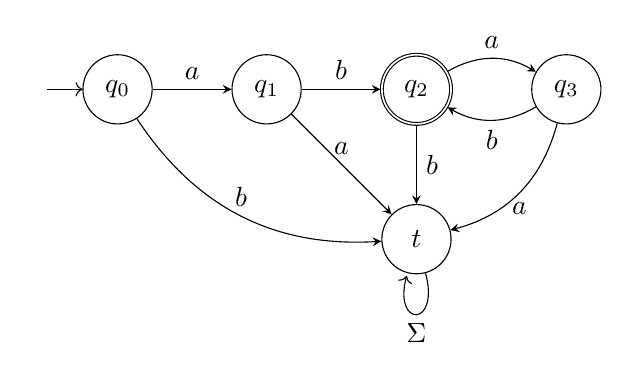
\begin{tikzpicture}
    \node (q0) [state, initial, initial text = {}] {$q_0$};
    \node (q1) [state, right = of q0] {$q_1$};
    \node (q2) [state, accepting, right = of q1] {$q_2$};
    \node (q3) [state, right = of q2] {$q_3$};
    \node (t) [state, below = of q2] {$t$};
    \path [-stealth]
    (q0) edge node[above] {$a$} (q1)
    (q0) edge[bend right] node[above] {$b$} (t)
    (q1) edge node[above] {$a$} (t)
    (q1) edge node[above] {$b$} (q2)
    (q2) edge[bend left] node[above] {$a$} (q3)
    (q2) edge node[right] {$b$} (t)
    (q3) edge[bend left] node[below] {$a$} (t)
    (q3) edge[bend left] node[below] {$b$} (q2)
    (t) edge[loop below] node[below] {$\Sigma$} ();
\end{tikzpicture}\\
We want words starting with $a$, ending with $b$, and having an alternating $a$-$b$ pattern. We don't want the empty word though; hence, we add $q_0$ and $q_1$.

\textbf{3:}

The automaton given is:\vspace{3mm}

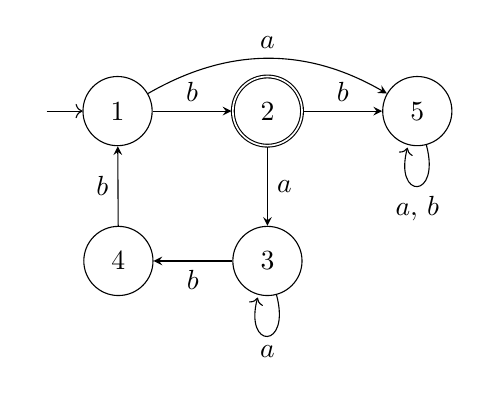
\begin{tikzpicture}
    \node (1) [state, initial, initial text = {}] {1};
    \node (2) [state, accepting, right = of 1] {2};
    \node (3) [state, below = of 2] {3};
    \node (4) [state, left = of 3] {4};
    \node (5) [state, right = of 2] {5};
    \path [-stealth]
        (1) edge node[above] {$b$} (2)
        (1) edge[bend left] node[above] {$a$} (5)
        (2) edge node[above] {$b$} (5)
        (2) edge node[right] {$a$} (3)
        (3) edge[loop below] node[below] {$a$} ()
        (3) edge node[below] {$b$} (4)
        (4) edge node[left] {$b$} (1)
        (5) edge[loop below] node[below] {$a,\, b$} ();
\end{tikzpicture}\\
5 is clearly a trap state. Let's ignore the paths leading to it. The first accepted word is ``b", and to get other words we need to go through the 2 $\rightarrow$ 3 $\rightarrow$ 4 $\rightarrow$ 1 $\rightarrow$ 2 cycle once ( $(abbb)^*$ ). However, we can go through the self-loop on 3 an arbitrary amount ($a^*$).

So, $L = b(a a^* bbb)^*$.

Define the following:

$\forall x, y, z \in Vars,\;\varphi_{bbb}(x, y, z) = S(x, y) \land S(y, z) \land Q_b(x) \land Q_b(y) \land Q_b(z)$

$\varphi_1 = \exists x.(first(x) \land Q_b(x))$ (since the word starts with a ``$b$").

$\varphi_2 = (\exists w.(first(w) \land \neg\, last(w))) \Rightarrow \exists x \exists y \exists z.(last(z) \land \varphi_{bbb}(x,\, y,\, z))$ (since if the word size is $>$ 1, the word has to end in a ``$bbb$").

$\varphi_3 = \forall x \forall y \forall z.(\;\varphi_{bbb}(x,\, y,\, z) \Rightarrow \exists w.(S(w, x) \land Q_a(w))\;)$ (Immediately before every occurrence of ``$bbb$'', there is a non-empty series of ``$a$''s).

$\varphi_4 = \forall w.(\; Q_a(w) \Rightarrow \forall x.(\;(Q_b(x) \land x < w) \Rightarrow (\; first(x) \lor \exists y \exists z.(\varphi_{bbb}(x, y, z))\;) \;)\;)$ (Before every ``$a$'', every occurrence of ``$b$'' before it is either the first letter or part of a ``$bbb$").

With all these, we claim our $L$ is exactly the language of $\varphi = \varphi_1 \land \varphi_2 \land \varphi_3 \land \varphi_4$ ! Try and figure out how - each $\varphi_i$ was coded such that together they provide us with all the necessary and sufficient properties to make $L$; however, saying that is rather vague.

Playing around with each $\varphi_i$ might provide you with a better understanding: just for an example, try and see how $\varphi_4' = \forall w.(\; Q_a(w) \Rightarrow \exists x.(\;Q_b(x) \land x < w \land (\; first(x) \lor \exists y \exists z.(\varphi_{bbb}(x, y, z))\;) \;)\;)$ won't work, even though it seems to be arguing something similar. Or, try to see how things change if, in our sub-formulae, we want to encode that immediately $after$ (not before) every ``bbb" not at the end, there are a non-empty number of `a's (and vice versa).
\end{flushleft}
\end{document}